\section{Logging delle attività}
All'interno del package di base della libreria è presente la classe \emph{singleton} \texttt{HostLoggerSupplier}, la cui istanza di \texttt{Logger} è stata impiegata sia all'interno delle classi della libreria che nelle classi d'avvio d'esempio allegate al progetto.
Tale istanza fornisce agli utenti una traccia sulle attività, siano esse di comunicazione, di gestione o di simulazione, svolte dagli applicativi riferiti ai nodi dell'architettura e notifica su tutti i possibili errori sollevati a tempo d'esecuzione.

Il sistema di logging comunica con l'utente tramite la console e tramite dei file in formato \texttt{.log} che vengono generati all'interno della directory da cui vengono eseguiti gli applicativi costruiti sfruttando la libreria sviluppata.

\begin{figure}[H]
    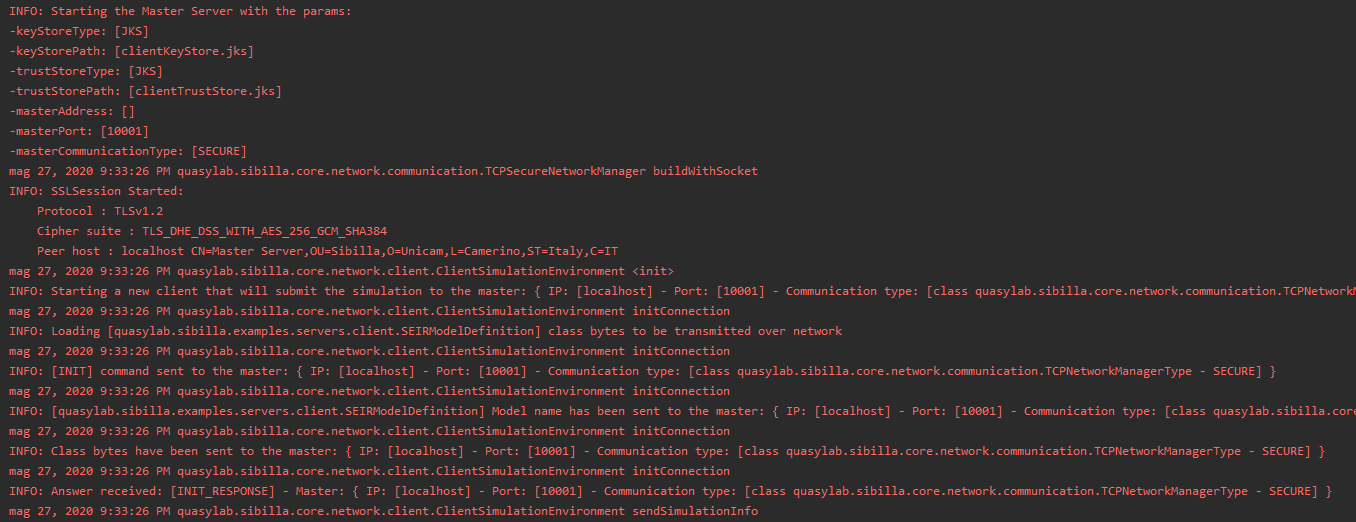
\includegraphics[width=\linewidth]{images/clientexamplelog.png}
    \captionsetup{justification=centering}
    \caption{Il log presente in un terminale in cui è stato avviato l'eseguibile del package \texttt{quasylab.sibilla.examples.servers.client}}
  \end{figure}